\chapter{色散、色差、点扩散与 MTF}
\label{ch:08}

\section{效果}
\label{sec:ch08-effect}

读完本章，你应能：
\begin{enumerate}
  \item 说明材料色散如何产生轴向色差与垂轴色差，以及为何结构光常选单色或窄带光源；
  \item 从 $\PSF$ 出发定义 $\mathrm{OTF}$ 与 $\MTF$，写出衍射限截止频率，并把离焦、像元采样等因素作为 $\MTF$ 级联相乘；
  \item 把「投影镜头 $\to$ 物面 $\to$ 相机镜头 $\to$ 像元」的链路 $\MTF$ 与第~\ref{ch:06}~章的调制幅 $M$ 和相位噪声 $\sigma_\varphi$ 联系起来；
  \item 解释边缘与高曲率处混合像素的成因；
  \item 为一台结构光设备选择条纹周期并做一份模糊预算。
\end{enumerate}

\section{原理}
\label{sec:ch08-principle}

\subsection{色散与色差}

透镜材料的折射率随波长变化，$n=n(\lambda)$，称为色散。可见光波段中，短波长折射率通常更大，因此薄透镜的焦距
\[
  \frac{1}{f(\lambda)}=\bigl(n(\lambda)-1\bigr)\Bigl(\frac{1}{r_1}-\frac{1}{r_2}\Bigr)
\]
随波长变化：蓝光焦距短于红光。（本章 $c$ 沿用第~\ref{ch:01}~章，表示弥散圆直径；第~\ref{ch:09}~章的 $c$ 表示光速。）由此产生两类色差：
\begin{itemize}
  \item \textbf{轴向色差}：不同波长的像面沿光轴前后错开。宽带照明下，任何一个像面都只对某一波段清晰，其余波段弥散，等效于叠加了波长相关的离焦。
  \item \textbf{垂轴色差（倍率色差）}：不同波长的放大率不同，视场边缘的像点按颜色径向错开。它在几何上等价于\emph{波长相关的径向畸变}（第~\ref{ch:02}~章）。
\end{itemize}
消色差设计用不同色散的玻璃组合，使两个波长焦点重合，剩余的二级光谱仍存在 \citep{HechtOptics}。

\textbf{对重建的含义。} 若相机按白光或某一波长标定，而工作时使用另一波长，焦距与畸变系数都会偏移，第~\ref{ch:07}~章已说明这会进入尺度项与畸变项。彩色编码结构光同时使用多个波长，每个颜色通道实际是一台内参略有不同的相机。

\textbf{单色源与带通。} 激光或窄带 LED 加带通滤光片可把色差压到近乎可忽略，并拒绝环境光（提高第~\ref{ch:05}~章的 $\SNR$）。代价：激光相干性高，带来散斑（第~\ref{ch:03}~章、第~\ref{ch:04}~章）；LED 带宽数十纳米，相干长度短，散斑弱，但仍有残余色差。口内设备常用蓝光 LED：短波长衍射截止更高、在牙体中穿透更浅（第~\ref{ch:06}~章），且带宽适中。

\subsection{PSF、OTF 与 MTF}

线性、空间不变近似下，像是物与 $\PSF$ 的卷积：
\begin{equation}
  I_{\mathrm{img}}(x,y)=\bigl(I_{\mathrm{obj}}*h\bigr)(x,y),
  \label{eq:ch08-conv}
\end{equation}
$h$ 为强度 $\PSF$。在频域中卷积变为相乘。设空间频率为 $(\xi,\eta)$（单位：周期/毫米），则
\begin{equation}
  \tilde I_{\mathrm{img}}(\xi,\eta)=H(\xi,\eta)\,\tilde I_{\mathrm{obj}}(\xi,\eta),\qquad
  H=\frac{\mathcal F\{h\}}{\mathcal F\{h\}(0,0)}.
  \label{eq:ch08-otf}
\end{equation}
$H$ 称为光学传递函数（OTF），其模 $|H|$ 即 $\MTF$，辐角为相位传递函数（PTF）。$\MTF$ 的物理意义直接：一个空间频率为 $\xi$、调制度为 $V_{\mathrm{in}}$ 的正弦图案经过系统后，调制度变为 $\MTF(\xi)V_{\mathrm{in}}$。这正是结构光关心的量。

\textbf{衍射限 MTF。} 非相干照明、圆形光瞳、无像差时 \citep{GoodmanFourierOptics}：
\begin{equation}
  \MTF(\xi)=\frac{2}{\pi}\Bigl[\arccos\hat\xi-\hat\xi\sqrt{1-\hat\xi^{2}}\Bigr],\qquad
  \hat\xi=\frac{\xi}{\xi_c},\qquad \xi_c=\frac{1}{\lambda N_F},
  \label{eq:ch08-diffmtf}
\end{equation}
$N_F$ 为工作 F 数（像方）。$\xi_c$ 以上 $\MTF$ 为零，任何信息都传不过去。例：$\lambda=450\,\mathrm{nm}$、$N_F=8$ 时 $\xi_c\approx278\,$周期/毫米；相机像元 $3\,\mu\mathrm{m}$ 的奈奎斯特频率约 $167\,$周期/毫米。

PTF 的非零部分（彗差等非对称像差造成）对结构光尤其危险：它让条纹整体平移，直接变成相位偏置，而不是对比度损失。

\subsection{MTF 级联}

若干独立的模糊环节串联时，总 $\PSF$ 为各 $\PSF$ 的卷积，总 $\MTF$ 为各 $\MTF$ 的乘积：
\begin{equation}
  \MTF_{\mathrm{sys}}(\xi)=\MTF_{\mathrm{diff}}(\xi)\cdot\MTF_{\mathrm{aber}}(\xi)\cdot\MTF_{\mathrm{defocus}}(\xi)\cdot\MTF_{\mathrm{pix}}(\xi)\cdots
  \label{eq:ch08-cascade}
\end{equation}
\begin{itemize}
  \item \textbf{离焦}：几何近似下弥散圆直径 $c$（第~\ref{ch:01}~章）对应的均匀圆盘 $\PSF$，其 $\MTF=2J_1(\pi c\xi)/(\pi c\xi)$，在 $\xi\approx1.22/c$ 处首次过零并出现\emph{对比度反转}（负值区相位翻转 $\pi$）。
  \item \textbf{像元孔径}：宽 $p$ 的方形像元相当于矩形积分，$\MTF_{\mathrm{pix}}=|\operatorname{sinc}(p\xi)|$；在奈奎斯特频率 $1/(2p)$ 处约为 $0.64$。
  \item \textbf{其他}：运动模糊（矩形核，沿运动方向）、传感器串扰、图像压缩等，皆可按同样方式相乘。
\end{itemize}
级联的直观结论：系统 $\MTF$ 永远不高于最差的一环，并且多个「看起来都还行」的环节相乘后会很快变差（图~\ref{fig:ch08-mtf}）。

\begin{figure}[htbp]
  \centering
  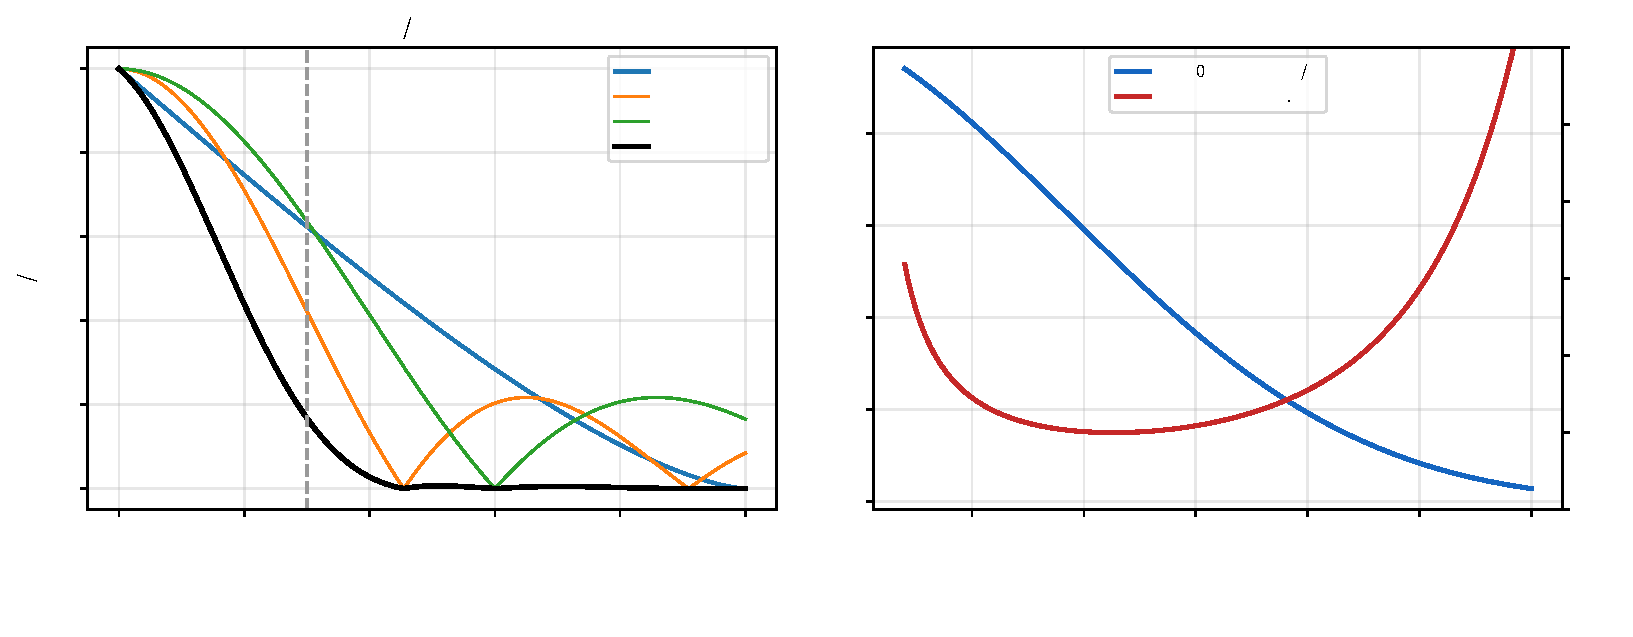
\includegraphics[width=0.98\textwidth]{fig-mtf-curve.pdf}
  \caption{左：衍射、离焦与像元 MTF 级联；右：链路 MTF 与相对深度噪声随条纹频率变化，存在最优区间（概念草图，非精确工程图）。}
  \label{fig:ch08-mtf}
\end{figure}

\subsection{链路 MTF、调制幅与相位噪声}

结构光中条纹经过两次成像：投影镜头把调制器上的图案成像到物面，相机镜头再把物面成像到传感器。物面的反射（含次表面散射）在中间又乘上一个「材料 $\MTF$」。设投影端条纹调制度为 $V_0$（第~\ref{ch:06}~章），相机所见调制度 $V=M/A$，平均灰度为 $A$，物面条纹频率为 $\xi$，则相机所见调制幅约为
\begin{equation}
  M(\xi)\approx A\,V_0\,\MTF_{\mathrm{proj}}(\xi)\,\MTF_{\mathrm{mat}}(\xi)\,\MTF_{\mathrm{cam}}(\xi).
  \label{eq:ch08-chain}
\end{equation}
代入第~\ref{ch:06}~章式~\eqref{eq:ch06-phase-noise}，$\sigma_\varphi\approx\sqrt{2/N}\,\sigma_I/M$。相位误差折算为物面横向位置误差为 $\delta x=\sigma_\varphi/(2\pi\xi)$，再经第~\ref{ch:07}~章的三角关系变成深度误差。于是
\begin{equation}
  \delta Z\ \propto\ \frac{1}{\xi\,\MTF_{\mathrm{link}}(\xi)}.
  \label{eq:ch08-tradeoff}
\end{equation}
提高条纹频率 $\xi$ 一方面使每弧度相位对应的位移更小（分母中的 $\xi$），另一方面使 $\MTF_{\mathrm{link}}$ 下降。二者乘积在某个中间频率处取最大，即深度噪声最小（图~\ref{fig:ch08-mtf} 右）。这给出选择条纹周期的光学依据，而不是「越密越好」。

\subsection{混合像素}

在深度不连续的边缘（牙齿轮廓、器械边缘），一个像元的 $\PSF$ 覆盖区域同时包含前景与背景。由于前后景的条纹相位不同，像元接收到的是两个复相量 $M_1e^{i\varphi_1}$ 与 $M_2e^{i\varphi_2}$ 按面积与亮度加权之和，求出的相位介于两者之间（甚至因相量抵消而 $M$ 很小），重建出漂浮在前后景之间的「飞点」。
高曲率表面虽然连续，但 $\PSF$ 覆盖区域内相位非线性变化，同样产生偏置，表现为尖锐边缘被「磨圆」、窄槽被「填浅」。$\PSF$ 越宽（离焦、低 $\MTF$），受影响的带宽越大。诊断特征：调制幅 $M$ 在边缘处骤降；相位梯度异常大。

\subsection{例：离焦怎样一步步吃掉调制度}

把模糊换算成调制度损失，就能直接接到第~\ref{ch:06}~章的相位噪声上。几何光学下，离焦 $\Delta z$ 在物方形成直径约
\[
  b\approx2\,\mathrm{NA}_o\,|\Delta z|
\]
的均匀圆斑（$\mathrm{NA}_o$ 为物方数值孔径；适用于离焦斑远大于衍射斑时）。均匀圆斑的 $\MTF$ 为
\[
  \MTF_{\mathrm{def}}(\xi)=\left|\frac{2J_1(\pi b\xi)}{\pi b\xi}\right|,
\]
小自变量时 $\approx1-(\pi b\xi)^2/8$。级联到式~\eqref{eq:ch08-cascade} 中，相机所见调制度 $V\approx V_0\cdot\MTF_{\mathrm{tot}}(\xi)$，相位噪声随 $1/V$ 增长。

\textbf{数量级示意。} 物方 $\mathrm{NA}_o=0.03$，条纹物方周期 $0.2\,\mathrm{mm}$（$\xi=5$ 周/mm）：
\begin{center}
\small
\begin{tabular}{cccc}
  \hline
  $|\Delta z|$ & $b$ & $\MTF_{\mathrm{def}}$ & $\sigma_\varphi$ 相对焦面\\
  \hline
  $0.5\,\mathrm{mm}$ & $30\,\mu\mathrm{m}$ & $0.97$ & $\times1.03$\\
  $1\,\mathrm{mm}$ & $60\,\mu\mathrm{m}$ & $0.89$ & $\times1.1$\\
  $2\,\mathrm{mm}$ & $120\,\mu\mathrm{m}$ & $0.62$ & $\times1.6$\\
  $3\,\mathrm{mm}$ & $180\,\mu\mathrm{m}$ & $0.28$ & $\times3.5$\\
  \hline
\end{tabular}
\end{center}
（$\pi b\xi=3.83$ 即 $b=244\,\mu\mathrm{m}$ 时 $\MTF$ 第一次降到零，条纹完全消失，之后出现反相的伪调制。）这里只算了相机侧离焦；投影侧同样离焦，两者相乘，实际下降更快。表中 $\Delta z=2\,\mathrm{mm}$ 一行与第~\ref{ch:01}~章算出的景深量级相当：景深边缘不是「清晰与模糊」的分界，而是相位噪声开始成倍增长的位置。

\subsection{例：混合像素的相量算一遍}

边缘像素中，前景面积占比 $\alpha$，前景与背景调制幅 $M_1$、$M_2$，相位差 $\Delta\varphi$。像素所得相量
\[
  \tilde M e^{i\tilde\varphi}=\alpha M_1e^{i\varphi_1}+(1-\alpha)M_2e^{i\varphi_2}.
\]
取 $\varphi_1=0$、$\alpha=0.5$、$M_1=3M_2$、$\Delta\varphi=1\,\mathrm{rad}$：
\[
  \tilde\varphi=\operatorname{atan2}\bigl(\sin1,\ 3+\cos1\bigr)=\operatorname{atan2}(0.841,\,3.540)\approx0.233\,\mathrm{rad}.
\]
面积各占一半，相位却只偏向背景 $0.233$ 而不是 $0.5\,\mathrm{rad}$：亮的一方「拉」住了相位。合成幅值 $\tilde M=0.5\times3.638M_2\approx1.82M_2$，比两者平均 $2M_2$ 低约 $9\%$，变化不大，因而单靠 $M$ 门限难以发现这种像素。若 $M_1=M_2$、$\Delta\varphi=\pi$，相量完全抵消，$\tilde M\to0$，此时 $M$ 门限能剔除它。所以混合像素有两种：抵消型（$M$ 骤降，易剔除）与偏置型（$M$ 基本正常，相位偏到一侧，需要用深度不连续检测或相位梯度判据）。

\subsection{去卷积能救回多少}

既然模糊是卷积（式~\eqref{eq:ch08-conv}），能否除以光学传递函数 复原？对结构光，关心的只是条纹基频 $\xi_0$ 处的幅度：除以 $\MTF(\xi_0)$ 能把 $M$ 恢复，但噪声同样被放大 $1/\MTF(\xi_0)$ 倍，$\SNR$ 不变，相位噪声也就不变。去卷积无法凭空恢复信噪比，它只在两种情况下有用：(i) 模糊在空间上变化（例如混合像素附近），复原能改善几何偏置；(ii) 需要的是图像外观而不是相位。对相位而言，真正的出口是让 $\MTF(\xi_0)$ 本身变大：选更长的条纹周期、更大的景深或对焦更准。

\section{限度}
\label{sec:ch08-limits}

\begin{itemize}
  \item 空间不变假设：真实镜头的 $\PSF$ 随视场与深度变化，$\MTF$ 应在多个视场点、多个深度分别给出；本章的单一曲线只是代表。
  \item 非相干成像假设：激光照明下系统对复振幅线性，传递函数是相干传递函数（截止频率为非相干的一半），且出现散斑。
  \item 级联相乘只对相互独立、线性的模糊环节成立；传感器饱和、伽马、二值化之后不再适用。
  \item 几何离焦 $\MTF$ 在弥散圆接近衍射斑时失效，需用波像差计算。
  \item 「材料 $\MTF$」是对次表面散射的粗略等效，忽略了它带来的相位偏移（第~\ref{ch:06}~章）。
\end{itemize}

\section{对象}
\label{sec:ch08-object}

\textbf{选条纹周期。} 设口内设备（数量级示意）：相机像元 $3\,\mu\mathrm{m}$、放大率 $0.3$，则物面像元约 $10\,\mu\mathrm{m}$；工作 F 数 $8$、蓝光。物面上条纹周期 $P_{\mathrm{obj}}$ 若取 $0.1\,\mathrm{mm}$（$10\,$周期/毫米），相当于每周期约 $10$ 个物面像元，像元 $\MTF$ 接近 $1$，衍射 $\MTF$ 仍高；但景深边缘弥散圆若达 $60\,\mu\mathrm{m}$（物面），离焦 $\MTF=2J_1(x)/x$ 在 $x=\pi c\xi\approx1.9$ 处约为 $0.6$，投影与相机两侧同时离焦则约 $0.36$，再叠加牙体散射，$M$ 可能只剩焦面处的三分之一左右。于是常见做法是：以\emph{景深边缘}而非焦面处的链路 $\MTF$ 来选周期，让边缘处 $M$ 仍高于展开可靠所需的阈值。

\textbf{模糊预算表。} 把每个环节在选定频率处的 $\MTF$ 列出（焦面 / 景深边缘两列）：投影衍射、投影离焦、材料、相机衍射、相机离焦、像元、运动。乘积给出 $M$ 的预期范围，再用式~\eqref{eq:ch06-phase-noise} 得到 $\sigma_\varphi$，用第~\ref{ch:07}~章的式~\eqref{eq:ch07-error} 得到 $\delta Z$。若结果超标，可从表中直接看出最差的一环：是离焦（需要更大景深或更小孔径）、是运动（需要更短曝光）、还是材料（需要更短波长或更低频率）。

\textbf{色差的实际影响。} 白光相机配蓝光投影：标定若用白光棋盘格，焦距与畸变系数会与蓝光工作状态略有差别，平面重建出现轻微碗形或尺度偏差。对策是用工作波长的照明进行标定，或在镜头设计中对工作波段做色差校正。

\section*{本章收束}
色散让焦距与畸变随波长变化，单色或窄带光源是结构光的常见选择。$\MTF$ 把模糊量化为「每个空间频率剩下多少调制度」，各环节级联相乘。调制幅 $M$ 是链路 $\MTF$ 的直接结果，因此条纹周期存在由光学决定的最优区间。边缘与高曲率处的混合像素来自 $\PSF$ 的有限宽度，是不可平均的系统误差。

\section{习题}
\label{sec:ch08-exercises}

\begin{enumerate}
  \item \textbf{（计算）} $\lambda=450\,\mathrm{nm}$、$N_F=5.6$ 与 $N_F=11$ 时衍射截止频率各为多少？对 $2.4\,\mu\mathrm{m}$ 像元，哪种情况下衍射成为奈奎斯特频率处的主导限制？
  \item \textbf{（计算）} 某频率处投影 $\MTF=0.7$、材料 $0.6$、相机 $0.8$、像元 $0.9$，投影端调制度 $V_0=0.9$，平均灰度 $A=120$。估算调制幅 $M$；若 $\sigma_I=2$、四步相移，求 $\sigma_\varphi$。
  \item \textbf{（重建场景）} 同一台设备在焦面处精度很好，在景深边缘噪声增加三倍以上，且条纹越密越明显。用 $\MTF$ 级联解释。
  \item \textbf{（重建场景）} 牙齿轮廓边缘一圈出现漂浮点，位于牙面与背景之间。原因是什么？给出基于 $M$ 和相位梯度的剔除规则。
  \item \textbf{（重建场景）} 换用另一颜色的投影光源后，未重新标定，平面重建出现轻微碗形。解释并给出对策。
  \item \textbf{（设计）} 由式~\eqref{eq:ch08-tradeoff}，若 $\MTF_{\mathrm{link}}(\xi)\approx1-\xi/\xi_0$（线性近似），求使 $\delta Z$ 最小的 $\xi$。
  \item \textbf{（诊断）} 相位误差图在某些区域条纹相位整体反转了约 $\pi$，而调制幅很低。可能是离焦 $\MTF$ 的什么现象？
  \item \textbf{（推导）} 由均匀圆斑的 $\MTF$ 小自变量展开，求 $\MTF_{\mathrm{def}}$ 降到 $0.9$ 时 $b\xi$ 的值，并给出对应的离焦量公式。
  \item \textbf{（计算）} 正文表中若条纹周期加长到 $0.4\,\mathrm{mm}$，$\Delta z=2\,\mathrm{mm}$ 时 $\MTF_{\mathrm{def}}$ 约为多少？代价是什么（结合第~\ref{ch:06}~章 $\delta d=P\sigma_\varphi/2\pi$）？
  \item \textbf{（口扫场景）} 牙齿邻接面边缘，前景牙面 $M_1=M_2$，$\alpha=0.3$，$\Delta\varphi=2\,\mathrm{rad}$。求合成相位与幅值；按 $P=16$ 像素换算为多少像素的投影坐标偏差？
  \item \textbf{（医学重建）} 内镜结构光中组织表面有一层液膜，使边缘出现强镜面高光（$M_1=10M_2$）。在 $\alpha$ 只有 $0.1$ 时，相位偏向高光一侧多少（$\Delta\varphi=1\,\mathrm{rad}$）？说明这对边缘几何的影响。
  \item \textbf{（C++/CUDA 实践）} 设计一个检测偏置型混合像素的 GPU 后处理：给出所用判据（相位梯度、深度跳变、$M$ 局部比值），以及邻域访问如何用共享内存实现。
\end{enumerate}

\section{习题讲解}
\label{sec:ch08-solutions}

\begin{enumerate}
  \item $\xi_c=1/(\lambda N_F)$：$N_F=5.6$ 时约 $397$，$N_F=11$ 时约 $202\,$周期/毫米。$2.4\,\mu\mathrm{m}$ 像元奈奎斯特约 $208\,$周期/毫米。$N_F=11$ 时截止频率已低于奈奎斯特，衍射主导。
  \item 链路 $\MTF=0.7\times0.6\times0.8\times0.9\approx0.30$；$M\approx120\times0.9\times0.30\approx33$。$\sigma_\varphi\approx\sqrt{2/4}\times2/33\approx0.043\,\mathrm{rad}$。
  \item 景深边缘离焦 $\MTF$ 大幅下降，投影与相机两侧同时离焦，且乘积随频率下降更快；$M$ 下降导致 $\sigma_\varphi$ 上升。条纹越密，离焦 $\MTF$ 越低，效应越强。
  \item 混合像素：$\PSF$ 跨越深度不连续，前后景相量叠加，求出中间相位。规则：剔除 $M$ 低于阈值（如局部中值的一定比例）或相位梯度超过可能表面坡度上限的像素；或检查邻域深度跳变后剔除边缘带。
  \item 轴向与垂轴色差：焦距与畸变系数随波长变化，标定参数不再匹配，残余畸变表现为碗形。对策：以工作波长重新标定，或使用色差校正的镜头。
  \item $\xi\,\MTF=\xi-\xi^2/\xi_0$ 在 $\xi=\xi_0/2$ 时取最大，此时 $\delta Z$ 最小。
  \item 离焦 $\MTF$ 过零后的负值区：对比度反转，相位翻转 $\pi$，同时幅值小。说明该区域严重离焦，应降低条纹频率或剔除。
  \item $1-x^2/8=0.9$ 得 $x=\pi b\xi\approx0.894$，$b\xi\approx0.285$；由 $b=2\mathrm{NA}_o|\Delta z|$，$|\Delta z|\approx0.142/(\mathrm{NA}_o\xi)$。$\mathrm{NA}_o=0.03$、$\xi=5$ 时约 $0.95\,\mathrm{mm}$，与表中 $1\,\mathrm{mm}$ 一行一致。
  \item $\xi=2.5$，$\pi b\xi=0.942$，$\MTF\approx1-0.111=0.89$（准确值约 $0.89$）。代价：$P$ 加倍，同样 $\sigma_\varphi$ 下 $\delta d$ 加倍；景深边缘处相位噪声减为约 $0.62/0.89$，综合后约 $2\times0.70=1.4$ 倍，焦面处则直接是 $2$ 倍。周期选择是景深与焦面精度的权衡。
  \item 相量 $0.3+0.7e^{2i}=0.3+0.7(-0.416+0.909i)=0.009+0.636i$，$\tilde\varphi\approx1.56\,\mathrm{rad}$，$\tilde M\approx0.64M_1$。相对前景偏 $1.56\,\mathrm{rad}$，约 $16\times1.56/6.28\approx4$ 像素。面积只占七成的背景主导了相位。
  \item $0.1\times10+0.9e^{i}=1+0.486+0.757i$，$\tilde\varphi=\operatorname{atan2}(0.757,1.486)\approx0.47\,\mathrm{rad}$。背景相位为 $1\,\mathrm{rad}$，合成相位被拉向高光约 $0.53\,\mathrm{rad}$：只占一成面积的高光把相位拉过了一半。边缘轮廓会向高光一侧「外扩」，表现为组织边缘鼓起。
  \item 判据：$|\nabla\varphi|$ 超过正常条纹梯度的若干倍；相邻深度跳变大于预设阈值；像素 $M$ 与邻域中位数之比偏离（抵消型低于 $0.5$）。实现：每个线程块把 $(16+2)\times(16+2)$ 的相位与 $M$ 瓦片载入共享内存（含一像素边框），同步后每线程计算梯度与邻域统计，标记可疑像素；被标记像素可剔除或在深度跳变两侧按最近侧填补。
\end{enumerate}
